\section{9 Nov 23 - Activity: Applying The Fast Fourier
Transform}\label{nov-23---activity-applying-the-fast-fourier-transform}

We were able to find the complex expansion coefficients for a signal
using a Fourier series. However, this method is only applicable to
periodic signals. Here we will introduce the Discrete Fourier Transform
(DFT) and the Fast Fourier Transform (FFT) which can be used to find the
complex expansion coefficients for any signal. The DFT is the discrete
analog to our expansion approach, the FFT improves the algorithmic
efficiency of the DFT, which we won't describe.

Let's remind ourselves of the Fourier series expansion for a periodic
signal \(x(t)\) with some period \(T_0\).

\begin{Shaded}
\begin{Highlighting}[]
\ImportTok{import}\NormalTok{ numpy }\ImportTok{as}\NormalTok{ np}
\ImportTok{import}\NormalTok{ matplotlib.pyplot }\ImportTok{as}\NormalTok{ plt}
\ImportTok{import}\NormalTok{ random}
\end{Highlighting}
\end{Shaded}

\subsection{A sinusoidal signal with a DC
offset}\label{a-sinusoidal-signal-with-a-dc-offset}

In this example we will use a sinusoidal signal with a DC offset. The
signal is defined as:

\[V(t) = A_0 \sin(2\pi f_0 t) + A_1 \sin(2\pi f_1 t) + A_2 \sin(2\pi f_2 t) + C\]

We create the signal a graph it.

\begin{Shaded}
\begin{Highlighting}[]
\KeywordTok{def}\NormalTok{ summed\_signal(t, A, f, C}\OperatorTok{=}\DecValTok{0}\NormalTok{):}
    \CommentTok{"""Creates a signal with multiple frequencies."""}
    \ControlFlowTok{return}\NormalTok{ A[}\DecValTok{0}\NormalTok{] }\OperatorTok{*}\NormalTok{ np.sin(}\DecValTok{2} \OperatorTok{*}\NormalTok{ np.pi }\OperatorTok{*}\NormalTok{ f[}\DecValTok{0}\NormalTok{]}\OperatorTok{*}\NormalTok{t) }\OperatorTok{+}\NormalTok{ A[}\DecValTok{1}\NormalTok{] }\OperatorTok{*}\NormalTok{ np.sin(}\DecValTok{2} \OperatorTok{*}\NormalTok{ np.pi }\OperatorTok{*}\NormalTok{ f[}\DecValTok{1}\NormalTok{]}\OperatorTok{*}\NormalTok{t) }\OperatorTok{+}\NormalTok{ A[}\DecValTok{2}\NormalTok{]}\OperatorTok{*}\NormalTok{np.sin(}\DecValTok{2} \OperatorTok{*}\NormalTok{ np.pi }\OperatorTok{*}\NormalTok{ f[}\DecValTok{2}\NormalTok{]}\OperatorTok{*}\NormalTok{t) }\OperatorTok{+}\NormalTok{ C}

\NormalTok{T0 }\OperatorTok{=} \FloatTok{0.5} \CommentTok{\# Signal period}
\NormalTok{N }\OperatorTok{=} \DecValTok{1000} \CommentTok{\# Number of samples}
\NormalTok{dt }\OperatorTok{=}\NormalTok{ T0}\OperatorTok{/}\NormalTok{N }\CommentTok{\# Time step}
\NormalTok{t }\OperatorTok{=}\NormalTok{ np.arange(}\DecValTok{0}\NormalTok{, }\DecValTok{3}\OperatorTok{*}\NormalTok{T0, dt)  }\CommentTok{\# Time points}

\NormalTok{f }\OperatorTok{=}\NormalTok{ np.array([}\DecValTok{1}\OperatorTok{/}\NormalTok{T0, }\DecValTok{2}\OperatorTok{/}\NormalTok{T0, }\DecValTok{3}\OperatorTok{/}\NormalTok{T0]) }\CommentTok{\# Frequencies}
\NormalTok{A }\OperatorTok{=}\NormalTok{ np.array([}\OperatorTok{{-}}\DecValTok{10}\NormalTok{, }\DecValTok{5}\NormalTok{, }\DecValTok{8}\NormalTok{]) }\CommentTok{\# Amplitudes}
\NormalTok{C }\OperatorTok{=} \DecValTok{4}  \CommentTok{\# DC Offset}

\NormalTok{summed }\OperatorTok{=}\NormalTok{ summed\_signal(t, A, f, C)}
\end{Highlighting}
\end{Shaded}

\begin{Shaded}
\begin{Highlighting}[]
\NormalTok{plt.figure(figsize}\OperatorTok{=}\NormalTok{(}\DecValTok{10}\NormalTok{, }\DecValTok{5}\NormalTok{))}

\NormalTok{plt.plot(t, summed)}

\NormalTok{plt.axvline(x}\OperatorTok{=}\DecValTok{0}\NormalTok{, color}\OperatorTok{=}\StringTok{\textquotesingle{}k\textquotesingle{}}\NormalTok{, linestyle}\OperatorTok{=}\StringTok{\textquotesingle{}{-}{-}\textquotesingle{}}\NormalTok{, lw}\OperatorTok{=}\DecValTok{2}\NormalTok{)}
\NormalTok{plt.axhline(y}\OperatorTok{=}\DecValTok{0}\NormalTok{, color}\OperatorTok{=}\StringTok{\textquotesingle{}k\textquotesingle{}}\NormalTok{, linestyle}\OperatorTok{=}\StringTok{\textquotesingle{}{-}{-}\textquotesingle{}}\NormalTok{, lw}\OperatorTok{=}\DecValTok{2}\NormalTok{)}

\NormalTok{plt.xlabel(}\StringTok{\textquotesingle{}Time (s)\textquotesingle{}}\NormalTok{)}
\NormalTok{plt.ylabel(}\StringTok{\textquotesingle{}Amplitude\textquotesingle{}}\NormalTok{)}

\NormalTok{plt.grid()}
\NormalTok{plt.tight\_layout()}
\end{Highlighting}
\end{Shaded}

\begin{figure}
\centering
\pandocbounded{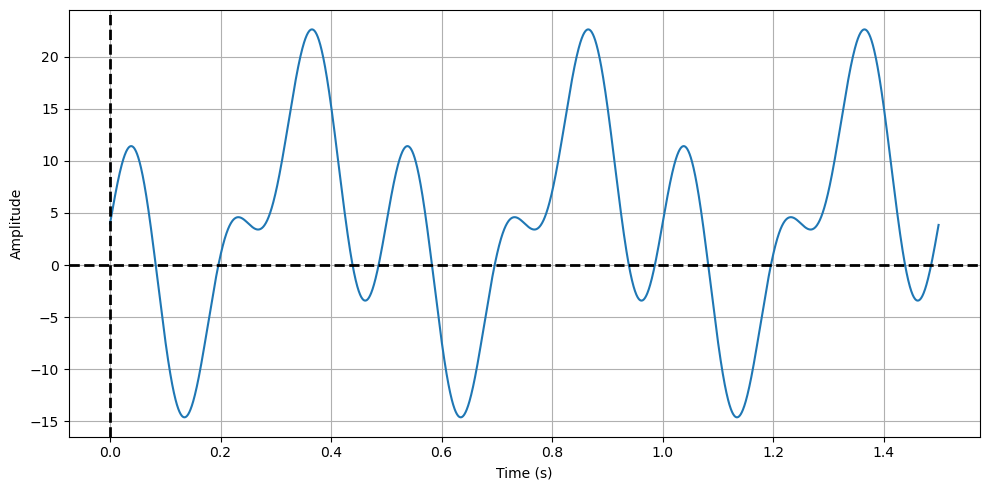
\includegraphics[keepaspectratio,alt={png}]{../images/activity-Waves-Applying_the_FFT_activity-Waves-Applying_the_FFT_tmp_4_0.png}}
\caption{png}
\end{figure}

\subsection{Extracting the Fourier
coefficients}\label{extracting-the-fourier-coefficients}

Let's extract the Fourier coefficients. We defined the base peridicity
\(T_0\) in the code above. If it was not changed it was 0.5 seconds. We
will use this to define the base frequency of the signal
\(f_0 = 1/T_0 = 1/0.5 = 2\) Hz. We have two more parts of the signal
from frequencies \(f_1 = 4\) Hz and \(f_2 = 6\) Hz. We will use the
Fourier series expansion to find the complex expansion coefficients
\(c_n\).

\begin{Shaded}
\begin{Highlighting}[]
\KeywordTok{def}\NormalTok{ compute\_cn(t\_, f, n):}
    \CommentTok{"""Computes the Fourier coefficient c\_n for a given time array.}
\CommentTok{    Assumes that the time array is evenly spaced. f is the signal }
\CommentTok{    and must have the same length as t."""}
\NormalTok{    dt }\OperatorTok{=}\NormalTok{ t\_[}\DecValTok{1}\NormalTok{] }\OperatorTok{{-}}\NormalTok{ t\_[}\DecValTok{0}\NormalTok{]}
    
    \ControlFlowTok{return} \DecValTok{1}\OperatorTok{/}\NormalTok{T0 }\OperatorTok{*}\NormalTok{ np.}\BuiltInTok{sum}\NormalTok{(f }\OperatorTok{*}\NormalTok{ np.exp(}\OperatorTok{{-}}\OtherTok{1j} \OperatorTok{*} \DecValTok{2} \OperatorTok{*}\NormalTok{ np.pi }\OperatorTok{*}\NormalTok{ n }\OperatorTok{*}\NormalTok{ t\_}\OperatorTok{/}\NormalTok{T0)) }\OperatorTok{*}\NormalTok{ dt}

\KeywordTok{def}\NormalTok{ compute\_power\_spectrum(t\_, f, N):}
    \CommentTok{"""Computes the power spectrum for a given time array and signal.}
\CommentTok{    Returns the coefficients from {-}N,N."""}
\NormalTok{    cn }\OperatorTok{=}\NormalTok{ np.zeros(}\DecValTok{2} \OperatorTok{*}\NormalTok{ N }\OperatorTok{+} \DecValTok{1}\NormalTok{, dtype}\OperatorTok{=}\BuiltInTok{complex}\NormalTok{)}
    \ControlFlowTok{for}\NormalTok{ n }\KeywordTok{in} \BuiltInTok{range}\NormalTok{(}\OperatorTok{{-}}\NormalTok{N , N }\OperatorTok{+} \DecValTok{1}\NormalTok{):}
\NormalTok{        cn[n }\OperatorTok{+}\NormalTok{ N] }\OperatorTok{=}\NormalTok{ compute\_cn(t\_, f, n)}
    \ControlFlowTok{return}\NormalTok{ cn}
\end{Highlighting}
\end{Shaded}

\begin{Shaded}
\begin{Highlighting}[]
\NormalTok{t\_ }\OperatorTok{=}\NormalTok{ np.arange(}\DecValTok{0}\NormalTok{, T0, dt)  }\CommentTok{\# Time points for a single period}
\NormalTok{N }\OperatorTok{=} \DecValTok{10} \CommentTok{\# Number of coefficients (2N+1)}
\NormalTok{freqs }\OperatorTok{=}\NormalTok{ np.arange(}\OperatorTok{{-}}\NormalTok{N, N}\OperatorTok{+}\DecValTok{1}\NormalTok{) }\OperatorTok{/}\NormalTok{ T0 }\CommentTok{\# Frequencies}

\NormalTok{cn }\OperatorTok{=}\NormalTok{ compute\_power\_spectrum(t\_, summed[:}\BuiltInTok{len}\NormalTok{(t\_)], N) }\CommentTok{\# Compute the coefficients}
\end{Highlighting}
\end{Shaded}

\begin{Shaded}
\begin{Highlighting}[]
\NormalTok{plt.figure(figsize}\OperatorTok{=}\NormalTok{(}\DecValTok{10}\NormalTok{, }\DecValTok{5}\NormalTok{))}

\NormalTok{plt.plot(freqs, np.}\BuiltInTok{abs}\NormalTok{(cn), }\StringTok{\textquotesingle{}{-}{-}rx\textquotesingle{}}\NormalTok{)}
\NormalTok{plt.xlabel(}\StringTok{\textquotesingle{}Frequency (Hz)\textquotesingle{}}\NormalTok{)}
\NormalTok{plt.ylabel(}\StringTok{\textquotesingle{}Amplitude\textquotesingle{}}\NormalTok{)}

\NormalTok{plt.axhline(y}\OperatorTok{=}\DecValTok{0}\NormalTok{, color}\OperatorTok{=}\StringTok{\textquotesingle{}k\textquotesingle{}}\NormalTok{, linestyle}\OperatorTok{=}\StringTok{\textquotesingle{}{-}{-}\textquotesingle{}}\NormalTok{, lw}\OperatorTok{=}\DecValTok{2}\NormalTok{)}
\NormalTok{plt.axvline(x}\OperatorTok{=}\DecValTok{0}\NormalTok{, color}\OperatorTok{=}\StringTok{\textquotesingle{}k\textquotesingle{}}\NormalTok{, linestyle}\OperatorTok{=}\StringTok{\textquotesingle{}{-}{-}\textquotesingle{}}\NormalTok{, lw}\OperatorTok{=}\DecValTok{2}\NormalTok{)}

\NormalTok{plt.tight\_layout()}
\NormalTok{plt.grid()}
\end{Highlighting}
\end{Shaded}

\begin{figure}
\centering
\pandocbounded{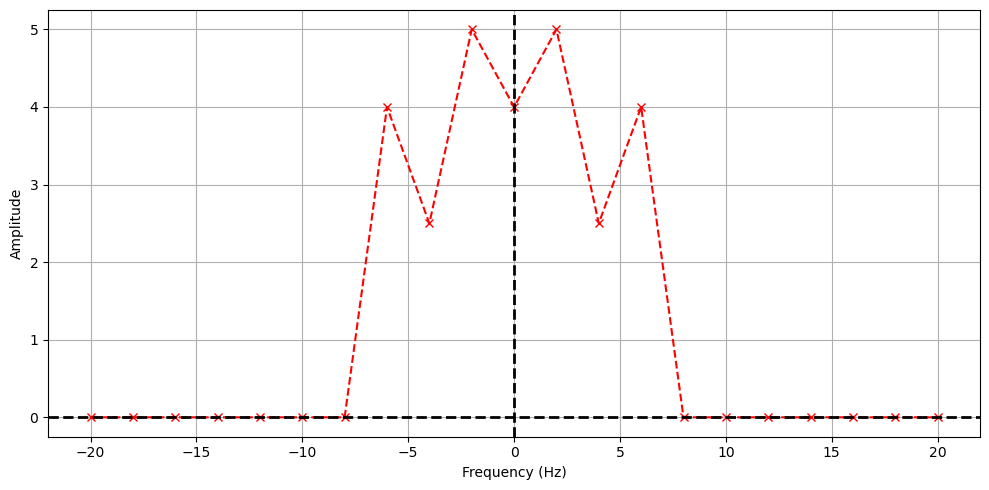
\includegraphics[keepaspectratio,alt={png}]{../images/activity-Waves-Applying_the_FFT_activity-Waves-Applying_the_FFT_tmp_8_0.png}}
\caption{png}
\end{figure}

\subsubsection{Where are the
coefficients?}\label{where-are-the-coefficients}

We get both positive and negative frequencies. But notice that if we add
the amplitudes of the matched positive and negative amplitudes, we get
the value of the coefficients in our constructed signal. This is because
the signal is real, so the coefficients are conjugate symmetric. We can
use this to plot the coefficients in a more intuitive way. Notice the DC
part of the signal is NOT conjugate symmetric, so we don't add it to the
negative frequency part.

\begin{Shaded}
\begin{Highlighting}[]
\NormalTok{plt.figure(figsize}\OperatorTok{=}\NormalTok{(}\DecValTok{10}\NormalTok{, }\DecValTok{5}\NormalTok{))}

\NormalTok{x }\OperatorTok{=}\NormalTok{ np.insert(freqs[N}\OperatorTok{+}\DecValTok{1}\NormalTok{:], }\DecValTok{0}\NormalTok{, freqs[N])}
\NormalTok{y }\OperatorTok{=}\NormalTok{ np.insert(}\DecValTok{2}\OperatorTok{*}\NormalTok{np.}\BuiltInTok{abs}\NormalTok{(cn[N}\OperatorTok{+}\DecValTok{1}\NormalTok{:]), }\DecValTok{0}\NormalTok{, np.}\BuiltInTok{abs}\NormalTok{(cn[N]))}

\NormalTok{plt.plot(x, y, }\StringTok{\textquotesingle{}{-}{-}rx\textquotesingle{}}\NormalTok{)}

\NormalTok{plt.title(}\StringTok{\textquotesingle{}Fourier Components\textquotesingle{}}\NormalTok{)}
\NormalTok{plt.xlabel(}\StringTok{\textquotesingle{}Frequency (Hz)\textquotesingle{}}\NormalTok{)}
\NormalTok{plt.ylabel(}\StringTok{\textquotesingle{}Amplitude\textquotesingle{}}\NormalTok{)}

\NormalTok{plt.axhline(y}\OperatorTok{=}\DecValTok{0}\NormalTok{, color}\OperatorTok{=}\StringTok{\textquotesingle{}k\textquotesingle{}}\NormalTok{, linestyle}\OperatorTok{=}\StringTok{\textquotesingle{}{-}{-}\textquotesingle{}}\NormalTok{, lw}\OperatorTok{=}\DecValTok{2}\NormalTok{)}
\NormalTok{plt.axvline(x}\OperatorTok{=}\DecValTok{0}\NormalTok{, color}\OperatorTok{=}\StringTok{\textquotesingle{}k\textquotesingle{}}\NormalTok{, linestyle}\OperatorTok{=}\StringTok{\textquotesingle{}{-}{-}\textquotesingle{}}\NormalTok{, lw}\OperatorTok{=}\DecValTok{2}\NormalTok{)}
\NormalTok{plt.xticks(np.arange(}\DecValTok{0}\NormalTok{,}\DecValTok{20}\NormalTok{,}\DecValTok{2}\NormalTok{))}

\NormalTok{plt.tight\_layout()}
\NormalTok{plt.grid()}
\end{Highlighting}
\end{Shaded}

\begin{figure}
\centering
\pandocbounded{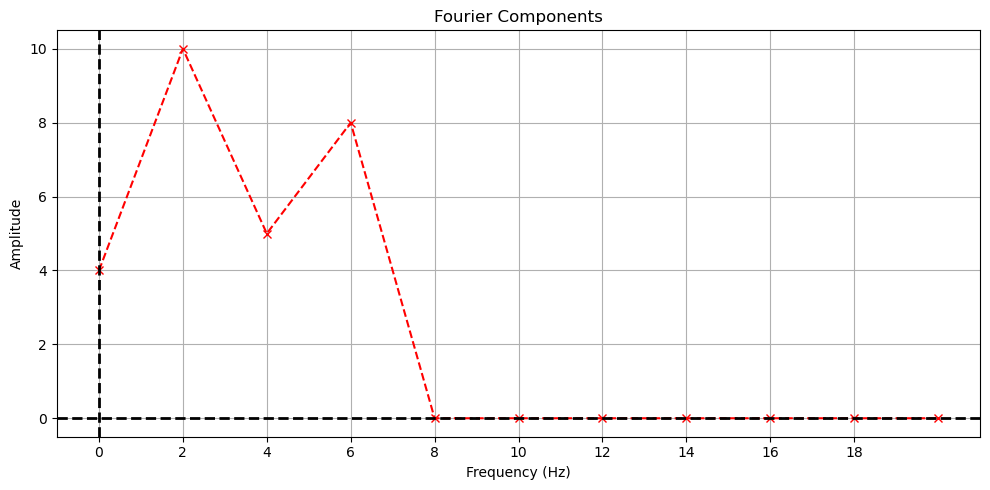
\includegraphics[keepaspectratio,alt={png}]{../images/activity-Waves-Applying_the_FFT_activity-Waves-Applying_the_FFT_tmp_10_0.png}}
\caption{png}
\end{figure}

\subsection{The Discrete Fourier
Transform}\label{the-discrete-fourier-transform}

One of the issues about the decomposition we have done is that it
assumes the signal is periodic. In practice, we often have signals that
are not periodic. For example, consider the signal below, which is a
wave packet that is not periodic. This signal is still of interest to us
and can often contain useful physics. But the techniques we have used so
far will not work for this signal.

\begin{Shaded}
\begin{Highlighting}[]
\CommentTok{\# Define the wave packet parameters}
\NormalTok{k0 }\OperatorTok{=} \DecValTok{5}  \CommentTok{\# central wavenumber}
\NormalTok{x0 }\OperatorTok{=} \DecValTok{0}  \CommentTok{\# initial position}
\NormalTok{spread }\OperatorTok{=} \DecValTok{1}  \CommentTok{\# spread of the packet}

\CommentTok{\# Create a space vector}
\NormalTok{x }\OperatorTok{=}\NormalTok{ np.linspace(}\OperatorTok{{-}}\DecValTok{10}\NormalTok{, }\DecValTok{10}\NormalTok{, }\DecValTok{1000}\NormalTok{)}

\CommentTok{\# Define the wave packet function}
\KeywordTok{def}\NormalTok{ wave\_packet(x, k0, x0, spread):}
    \ControlFlowTok{return}\NormalTok{ np.exp(}\OperatorTok{{-}}\FloatTok{0.5} \OperatorTok{*}\NormalTok{ ((x }\OperatorTok{{-}}\NormalTok{ x0) }\OperatorTok{/}\NormalTok{ spread) }\OperatorTok{**} \DecValTok{2}\NormalTok{) }\OperatorTok{*}\NormalTok{ np.cos(k0 }\OperatorTok{*}\NormalTok{ x)}

\CommentTok{\# Calculate the wave packet}
\NormalTok{psi }\OperatorTok{=}\NormalTok{ wave\_packet(x, k0, x0, spread)}

\CommentTok{\# Plot the wave packet}
\NormalTok{plt.figure(figsize}\OperatorTok{=}\NormalTok{(}\DecValTok{10}\NormalTok{, }\DecValTok{5}\NormalTok{))}
\NormalTok{plt.plot(x, psi)}
\NormalTok{plt.title(}\StringTok{\textquotesingle{}Wave Packet\textquotesingle{}}\NormalTok{)}
\NormalTok{plt.xlabel(}\StringTok{\textquotesingle{}Position\textquotesingle{}}\NormalTok{)}
\NormalTok{plt.ylabel(}\StringTok{\textquotesingle{}Amplitude\textquotesingle{}}\NormalTok{)}
\NormalTok{plt.grid(}\VariableTok{True}\NormalTok{)}
\NormalTok{plt.tight\_layout()}
\end{Highlighting}
\end{Shaded}

\begin{figure}
\centering
\pandocbounded{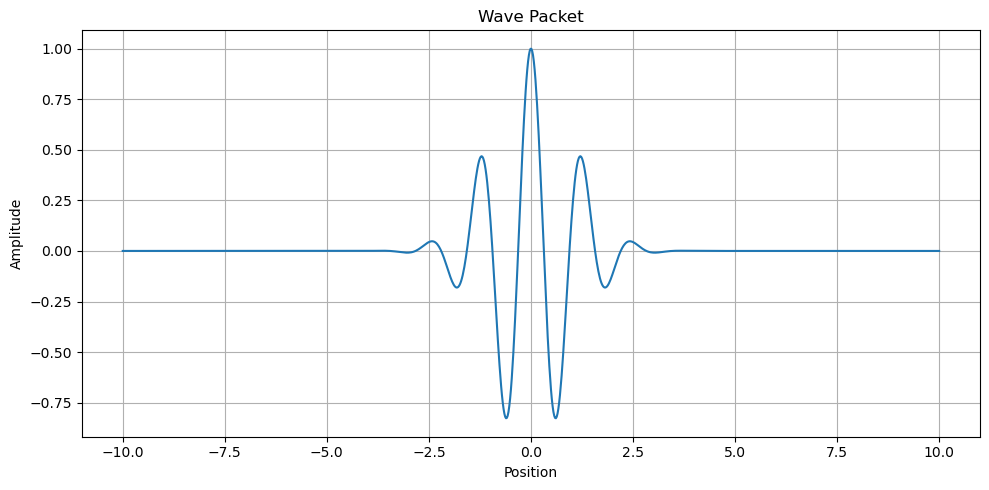
\includegraphics[keepaspectratio,alt={png}]{../images/activity-Waves-Applying_the_FFT_activity-Waves-Applying_the_FFT_tmp_12_0.png}}
\caption{png}
\end{figure}

\subsubsection{Enter the Discrete Fourier
Transform}\label{enter-the-discrete-fourier-transform}

The
\href{https://en.wikipedia.org/wiki/Discrete_Fourier_transform}{Discrete
Fourier Transform (DFT)} is a way to decompose a signal into a sum of
sinusoids, but it does not require the signal to be periodic. You can
think of it as a discretization of the processes we developed earlier.
The expansion of the signal is still as it was before, but we understand
it represents a finite number of samples of the signal:

\[V(t) = \sum_{n=0}^{N-1} c_n e^{i n \omega t}.\]

However, we now understand that the signal is only defined at discrete
times \(t_n = n \Delta t\) where \(\Delta t\) is the time between
samples. We can then write the Fourier coefficients as:

\[c_n \approx \frac{1}{T_0} \sum_{k=0}^{N-1} V(t_k)e^{-i n \omega t_k} \Delta t\]

where \(V(t_k)\) is the value of the signal at time \(t_k\) and
\(T_0 = N \Delta t\) is the total time of the signal.

\subsubsection{Assumptions}\label{assumptions}

In doing this, we are not creating a tool that will always work. We note
a few important assumptions and caveats:

\begin{enumerate}
\def\labelenumi{\arabic{enumi}.}
\item
  \textbf{Periodicity}: The DFT assumes that the input signal is
  periodic and that the period is exactly the length of the sample
  window. This means that the finite sequence of data points provided to
  the DFT is one period of a periodic signal that repeats indefinitely.
\item
  \textbf{Discrete Samples}: The signal being transformed is assumed to
  be sampled at discrete intervals. The DFT operates on these discrete
  samples and does not account for any data between the samples.
\item
  \textbf{Finite Duration}: The DFT is designed to handle signals of
  finite duration. The signal is assumed to have a finite number of
  samples, which is the number of points in the DFT.
\item
  \textbf{Equally-Spaced Samples}: The samples are assumed to be evenly
  spaced in time (or space, depending on the context of the signal).
  This uniform spacing is critical because non-uniformly spaced samples
  would require a different transform, such as the Non-uniform Discrete
  Fourier Transform (NDFT).
\end{enumerate}

\subsection{The Fast Fourier
Transform}\label{the-fast-fourier-transform}

While we can use the DFT directly, the FFT is more efficient and has
become the standard way to perform these analyses. The code to have
\texttt{numpy.fft} perform the FFT is pretty simple. But there's many
things to understand about the FFT and a variety of ways to produce
spurious and incoherent results. Let's use the simple signal we have
above to make go through an analysis.

\subsubsection{\texorpdfstring{The FFT in
\texttt{numpy.fft}}{The FFT in numpy.fft}}\label{the-fft-in-numpy.fft}

We start by importing the libraries. Then we need to:

\begin{enumerate}
\def\labelenumi{\arabic{enumi}.}
\tightlist
\item
  Define the time array
\item
  Define the signal
\item
  Perform the FFT using \texttt{numpy.fft.fft} (\emph{We imported
  \texttt{numpy.fft} below, so you can call \texttt{fft} directly.})
\item
  Plot the coefficients
\item
  Plot the power spectrum
\end{enumerate}

\begin{Shaded}
\begin{Highlighting}[]
\ImportTok{from}\NormalTok{ numpy.fft }\ImportTok{import}\NormalTok{ fft, fftfreq}

\NormalTok{plt.figure(figsize}\OperatorTok{=}\NormalTok{(}\DecValTok{6}\NormalTok{, }\DecValTok{4}\NormalTok{))}
\NormalTok{plt.plot(t, summed)}

\NormalTok{plt.title(}\StringTok{\textquotesingle{}Summed Signal\textquotesingle{}}\NormalTok{)}
\NormalTok{plt.xlabel(}\StringTok{\textquotesingle{}Time (s)\textquotesingle{}}\NormalTok{)}
\NormalTok{plt.ylabel(}\StringTok{\textquotesingle{}Amplitude\textquotesingle{}}\NormalTok{)}

\NormalTok{plt.tight\_layout()}
\NormalTok{plt.grid()}
\end{Highlighting}
\end{Shaded}

\begin{figure}
\centering
\pandocbounded{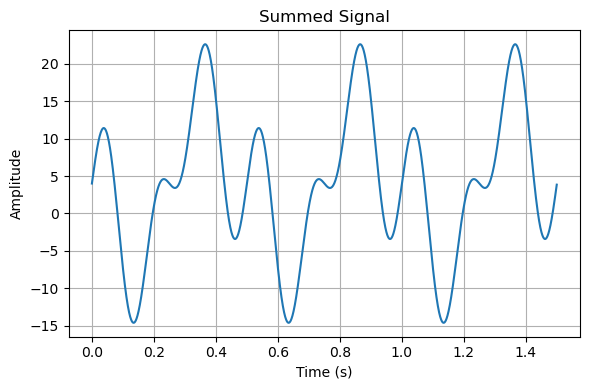
\includegraphics[keepaspectratio,alt={png}]{../images/activity-Waves-Applying_the_FFT_activity-Waves-Applying_the_FFT_tmp_16_0.png}}
\caption{png}
\end{figure}

\subsubsection{Computing and plotting Fourier
Coefficients}\label{computing-and-plotting-fourier-coefficients}

We now use \texttt{fft} to calculate the Fourier transform of the signal
and \texttt{fftfreq} to calculate the frequencies associated with the
transform. This is a standard way to do this analysis, but the most
common mistakes involve the frequencies. Because it is a real signal, we
don't worry about the negative frequencies, they are duplicate
information. The amplitudes of the non DC frequencies are doubled like
before to illustrate the Fourier coefficients.

\begin{Shaded}
\begin{Highlighting}[]
\NormalTok{t\_ }\OperatorTok{=}\NormalTok{ np.arange(}\DecValTok{0}\NormalTok{, T0, dt)  }\CommentTok{\# Time points for a single period}
\NormalTok{one\_cycle }\OperatorTok{=}\NormalTok{ summed[:}\BuiltInTok{len}\NormalTok{(t\_)] }\CommentTok{\# One cycle of the summed signal}
\NormalTok{N }\OperatorTok{=} \BuiltInTok{int}\NormalTok{(T0}\OperatorTok{/}\NormalTok{dt}\OperatorTok{/}\DecValTok{2}\NormalTok{) }\CommentTok{\# Maximum number of coefficients}

\NormalTok{fft\_summed }\OperatorTok{=}\NormalTok{ fft(one\_cycle)}
\NormalTok{freqs\_array }\OperatorTok{=}\NormalTok{ fftfreq(}\BuiltInTok{len}\NormalTok{(one\_cycle), dt)}

\NormalTok{x }\OperatorTok{=}\NormalTok{ freqs\_array[:N]}
\NormalTok{y }\OperatorTok{=}\NormalTok{ np.insert(}\DecValTok{2}\OperatorTok{*}\NormalTok{np.}\BuiltInTok{abs}\NormalTok{(fft\_summed[}\DecValTok{1}\NormalTok{:N]), }\DecValTok{0}\NormalTok{, np.}\BuiltInTok{abs}\NormalTok{(fft\_summed[}\DecValTok{0}\NormalTok{]))}
\end{Highlighting}
\end{Shaded}

\begin{Shaded}
\begin{Highlighting}[]
\NormalTok{plt.plot(x, y, }\StringTok{\textquotesingle{}{-}{-}rx\textquotesingle{}}\NormalTok{)}

\NormalTok{plt.title(}\StringTok{\textquotesingle{}Signal FFT (numpy.fft)\textquotesingle{}}\NormalTok{)}
\NormalTok{plt.xlabel(}\StringTok{\textquotesingle{}Frequency (Hz)\textquotesingle{}}\NormalTok{)}
\NormalTok{plt.ylabel(}\StringTok{\textquotesingle{}Amplitude\textquotesingle{}}\NormalTok{)}

\NormalTok{plt.axhline(y}\OperatorTok{=}\DecValTok{0}\NormalTok{, color}\OperatorTok{=}\StringTok{\textquotesingle{}k\textquotesingle{}}\NormalTok{, linestyle}\OperatorTok{=}\StringTok{\textquotesingle{}{-}{-}\textquotesingle{}}\NormalTok{, lw}\OperatorTok{=}\DecValTok{2}\NormalTok{)}
\NormalTok{plt.axvline(x}\OperatorTok{=}\DecValTok{0}\NormalTok{, color}\OperatorTok{=}\StringTok{\textquotesingle{}k\textquotesingle{}}\NormalTok{, linestyle}\OperatorTok{=}\StringTok{\textquotesingle{}{-}{-}\textquotesingle{}}\NormalTok{, lw}\OperatorTok{=}\DecValTok{2}\NormalTok{)}

\NormalTok{plt.xlim(}\DecValTok{0}\NormalTok{, }\DecValTok{20}\NormalTok{)}
\NormalTok{plt.xticks(np.arange(}\DecValTok{0}\NormalTok{,}\DecValTok{20}\NormalTok{,}\DecValTok{2}\NormalTok{))}

\NormalTok{plt.grid()}
\end{Highlighting}
\end{Shaded}

\begin{figure}
\centering
\pandocbounded{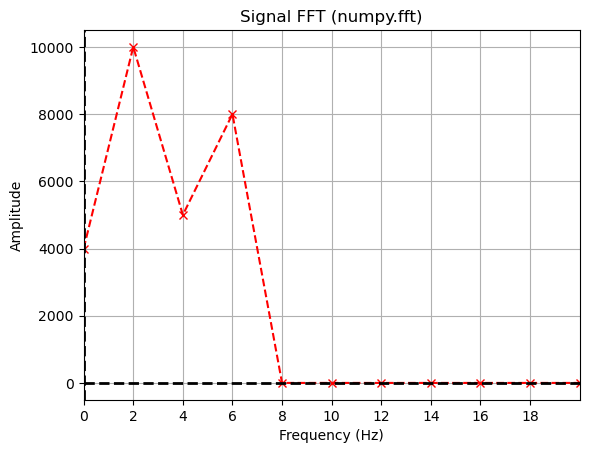
\includegraphics[keepaspectratio,alt={png}]{../images/activity-Waves-Applying_the_FFT_activity-Waves-Applying_the_FFT_tmp_19_0.png}}
\caption{png}
\end{figure}

Notice the FFT looks precisely the same as before. But the Amplitudes
are scaled differently. The total amplitude is not the same, but the
relative values are still meaningful. If the maximum amplitude is scaled
to the amplitude we had before, then the signal would look the same.
However, it's typical to instead plot these scaled in some way. The most
common way is to either scale them by the maximum amplitude or the sum
of all the amplitudes. Each have their own purpose and meaning. Below we
plot them both for comparison.

\begin{Shaded}
\begin{Highlighting}[]
\NormalTok{plt.figure(figsize}\OperatorTok{=}\NormalTok{(}\DecValTok{12}\NormalTok{, }\DecValTok{4}\NormalTok{))}

\NormalTok{plt.subplot(}\DecValTok{121}\NormalTok{)}
\NormalTok{plt.plot(x, y}\OperatorTok{/}\NormalTok{np.}\BuiltInTok{max}\NormalTok{(y), }\StringTok{\textquotesingle{}o\textquotesingle{}}\NormalTok{)}
\NormalTok{plt.xlim(}\DecValTok{0}\NormalTok{,}\DecValTok{20}\NormalTok{)}
\NormalTok{plt.xticks(np.arange(}\DecValTok{0}\NormalTok{,}\DecValTok{20}\NormalTok{,}\DecValTok{2}\NormalTok{))}

\NormalTok{plt.title(}\StringTok{\textquotesingle{}Signal FFT (normed by max)\textquotesingle{}}\NormalTok{)}
\NormalTok{plt.xlabel(}\StringTok{\textquotesingle{}Frequency (Hz)\textquotesingle{}}\NormalTok{)}
\NormalTok{plt.ylabel(}\StringTok{\textquotesingle{}Amplitude (Arb. Units)\textquotesingle{}}\NormalTok{)}

\NormalTok{plt.axhline(y}\OperatorTok{=}\DecValTok{0}\NormalTok{, color}\OperatorTok{=}\StringTok{\textquotesingle{}k\textquotesingle{}}\NormalTok{, linestyle}\OperatorTok{=}\StringTok{\textquotesingle{}{-}{-}\textquotesingle{}}\NormalTok{, lw}\OperatorTok{=}\DecValTok{2}\NormalTok{)}
\NormalTok{plt.axvline(x}\OperatorTok{=}\DecValTok{0}\NormalTok{, color}\OperatorTok{=}\StringTok{\textquotesingle{}k\textquotesingle{}}\NormalTok{, linestyle}\OperatorTok{=}\StringTok{\textquotesingle{}{-}{-}\textquotesingle{}}\NormalTok{, lw}\OperatorTok{=}\DecValTok{2}\NormalTok{)}

\NormalTok{plt.grid()}

\NormalTok{plt.subplot(}\DecValTok{122}\NormalTok{)}
\NormalTok{plt.plot(x, np.}\BuiltInTok{abs}\NormalTok{(y)}\OperatorTok{/}\NormalTok{np.}\BuiltInTok{sum}\NormalTok{(y), }\StringTok{\textquotesingle{}o\textquotesingle{}}\NormalTok{)}
\NormalTok{plt.xlim(}\DecValTok{0}\NormalTok{,}\DecValTok{20}\NormalTok{)}
\NormalTok{plt.xticks(np.arange(}\DecValTok{0}\NormalTok{,}\DecValTok{20}\NormalTok{,}\DecValTok{2}\NormalTok{))}

\NormalTok{plt.title(}\StringTok{\textquotesingle{}Signal FFT (normed by total)\textquotesingle{}}\NormalTok{)}
\NormalTok{plt.xlabel(}\StringTok{\textquotesingle{}Frequency (Hz)\textquotesingle{}}\NormalTok{)}
\NormalTok{plt.ylabel(}\StringTok{\textquotesingle{}Amplitude (Arb. Units)\textquotesingle{}}\NormalTok{)}

\NormalTok{plt.axhline(y}\OperatorTok{=}\DecValTok{0}\NormalTok{, color}\OperatorTok{=}\StringTok{\textquotesingle{}k\textquotesingle{}}\NormalTok{, linestyle}\OperatorTok{=}\StringTok{\textquotesingle{}{-}{-}\textquotesingle{}}\NormalTok{, lw}\OperatorTok{=}\DecValTok{2}\NormalTok{)}
\NormalTok{plt.axvline(x}\OperatorTok{=}\DecValTok{0}\NormalTok{, color}\OperatorTok{=}\StringTok{\textquotesingle{}k\textquotesingle{}}\NormalTok{, linestyle}\OperatorTok{=}\StringTok{\textquotesingle{}{-}{-}\textquotesingle{}}\NormalTok{, lw}\OperatorTok{=}\DecValTok{2}\NormalTok{)}

\NormalTok{plt.tight\_layout()}
\NormalTok{plt.grid()}
\end{Highlighting}
\end{Shaded}

\begin{figure}
\centering
\pandocbounded{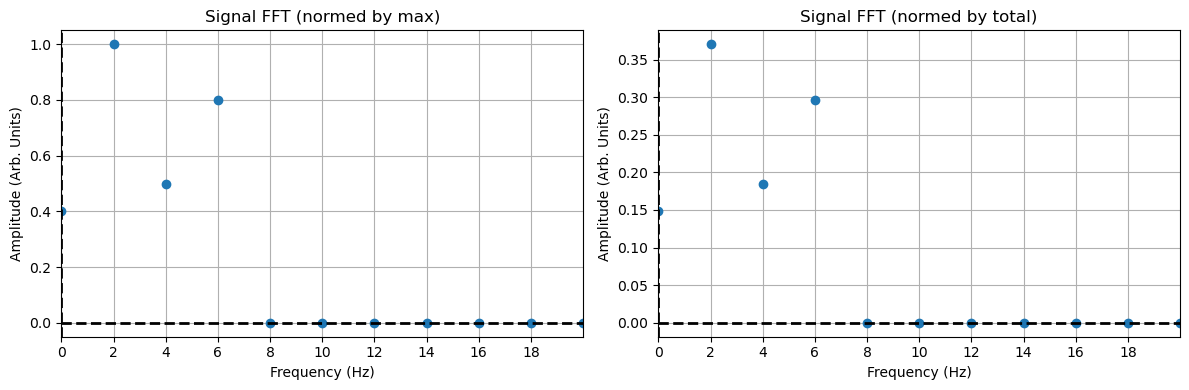
\includegraphics[keepaspectratio,alt={png}]{../images/activity-Waves-Applying_the_FFT_activity-Waves-Applying_the_FFT_tmp_21_0.png}}
\caption{png}
\end{figure}

\subsubsection{Investigating the FFT}\label{investigating-the-fft}

Now that you have developed some code and some conceptual understanding
of the FFT process, let's investigate some of the more nuanced aspects.

\textbf{✅ Do this}

\begin{enumerate}
\def\labelenumi{\arabic{enumi}.}
\tightlist
\item
  Complete the power spectrum analysis for the following signals that
  you construct:

  \begin{itemize}
  \tightlist
  \item
    Your signals have two frequencies that are close together (competing
    frequencies)
  \item
    Your signal has frequencies that are not integer multiples of the
    sampling rate (aliasing)
  \end{itemize}
\item
  Use \texttt{fft} to do these analyses and plot the spectra.
\item
  For the first case, what seems to be needed to resolve the two
  frequencies?
\item
  For the second case, what happens when the frequency is not an integer
  multiple of the sampling rate? What does this mean when signals have
  two frequencies that are not integer multiples of each other or the
  sampling rate?
\end{enumerate}

\begin{Shaded}
\begin{Highlighting}[]
\CommentTok{\#\# your code here}
\end{Highlighting}
\end{Shaded}
